%%%%%%%%%%%%%%%%%%%%%%%%%%%%%%%%%%%%%%%%%
% Beamer Presentation
% LaTeX Template
% Version 1.0 (10/11/12)
%
% This template has been downloaded from:
% http://www.LaTeXTemplates.com
%
% License:
% CC BY-NC-SA 3.0 (http://creativecommons.org/licenses/by-nc-sa/3.0/)
%
%%%%%%%%%%%%%%%%%%%%%%%%%%%%%%%%%%%%%%%%%

%----------------------------------------------------------------------------------------
%	PACKAGES AND THEMES
%----------------------------------------------------------------------------------------

\documentclass{beamer}

\mode<presentation> {

% The Beamer class comes with a number of default slide themes
% which change the colors and layouts of slides. Below this is a list
% of all the themes, uncomment each in turn to see what they look like.

%\usetheme{default}
%\usetheme{AnnArbor}
%\usetheme{Antibes}
%\usetheme{Bergen}
%\usetheme{Berkeley}
%\usetheme{Berlin}
%\usetheme{Boadilla}
%\usetheme{CambridgeUS}
%\usetheme{Copenhagen}
%\usetheme{Darmstadt}
%\usetheme{Dresden}
%\usetheme{Frankfurt}
%\usetheme{Goettingen}
%\usetheme{Hannover}
%\usetheme{Ilmenau}
%\usetheme{JuanLesPins}
%\usetheme{Luebeck}
\usetheme{Madrid}
%\usetheme{Malmoe}
%\usetheme{Marburg}
%\usetheme{Montpellier}
%\usetheme{PaloAlto}
%\usetheme{Pittsburgh}
%\usetheme{Rochester}
%\usetheme{Singapore}
%\usetheme{Szeged}
%\usetheme{Warsaw}

% As well as themes, the Beamer class has a number of color themes
% for any slide theme. Uncomment each of these in turn to see how it
% changes the colors of your current slide theme.

%\usecolortheme{albatross}
%\usecolortheme{beaver}
%\usecolortheme{beetle}
%\usecolortheme{crane}
%\usecolortheme{dolphin}
%\usecolortheme{dove}
%\usecolortheme{fly}
%\usecolortheme{lily}
%\usecolortheme{orchid}
%\usecolortheme{rose}
%\usecolortheme{seagull}
%\usecolortheme{seahorse}
%\usecolortheme{whale}
%\usecolortheme{wolverine}

%\setbeamertemplate{footline} % To remove the footer line in all slides uncomment this line
%\setbeamertemplate{footline}[page number] % To replace the footer line in all slides with a simple slide count uncomment this line

%\setbeamertemplate{navigation symbols}{} % To remove the navigation symbols from the bottom of all slides uncomment this line
}
\graphicspath{{Images/}}
\usepackage{graphicx} % Allows including images
\usepackage{booktabs} % Allows the use of \toprule, \midrule and \bottomrule in tables

\usepackage[utf8]{inputenc}% A modifier en fonction du codage d'entrée
\usepackage[T1]{fontenc}
\usepackage{lmodern}% Ou autre fonte

 \usepackage[french]{babel}
%----------------------------------------------------------------------------------------
%	TITLE PAGE
%----------------------------------------------------------------------------------------

\title[Magic Tiles]{Soutenance Développement Mobile : Magic Tiles} % The short title appears at the bottom of every slide, the full title is only on the title page

\author{Kamarouzamane Combo \& Hajanirina Randimbisoa} % Your name

\institute{\normalsize{M1 Informatique Université de la Réunion}}

\date{\today} % Date, can be changed to a custom date

\begin{document}

\begin{frame}
\titlepage % Print the title page as the first slide
\end{frame}

\begin{frame}
\frametitle{Sommaire} % Table of contents slide, comment this block out to remove it
\tableofcontents % Throughout your presentation, if you choose to use \section{} and \subsection{} commands, these will automatically be printed on this slide as an overview of your presentation
\end{frame}

%----------------------------------------------------------------------------------------
%	PRESENTATION SLIDES
%----------------------------------------------------------------------------------------

%-------------------------------------------------------------------------------------------------------------------------------------------------------------
\section{Introduction}
%-------------------------------------------------------------------------------------------------------------------------------------------------------------

%\subsection{Subsection Example} % A subsection can be created just before a set of slides with a common theme to further break down your presentation into chunks


\begin{frame}
  \frametitle{Introduction}
  \begin{block}{Objectif}
    \begin{itemize}
    \item {Créer une application mobile sur Android et iOS}
    \end{itemize}
  \end{block}
    \begin{block}{Contraintes}
    \begin{itemize}
    \item {Changement de configuration}
    \item {Géolocalisation}
    \item {Utiliser un capteur}
    \item {Utilisation d' au moins un geste courant non-trivial}
    \item {Ajouter du son}
    \end{itemize}
  \end{block}
\end{frame}


%-------------------------------------------------------------------------------------------------------------------------------------------------------------
\section{Présentation du jeu}
%-------------------------------------------------------------------------------------------------------------------------------------------------------------

\begin{frame}
  \frametitle{Présentation du jeu}
\begin{block}{Principe} 
    \begin{itemize}
         \item {Le jeu Magic Tiles est un jeu de modélisation et de simulation des touches de piano}
     \begin{center}
      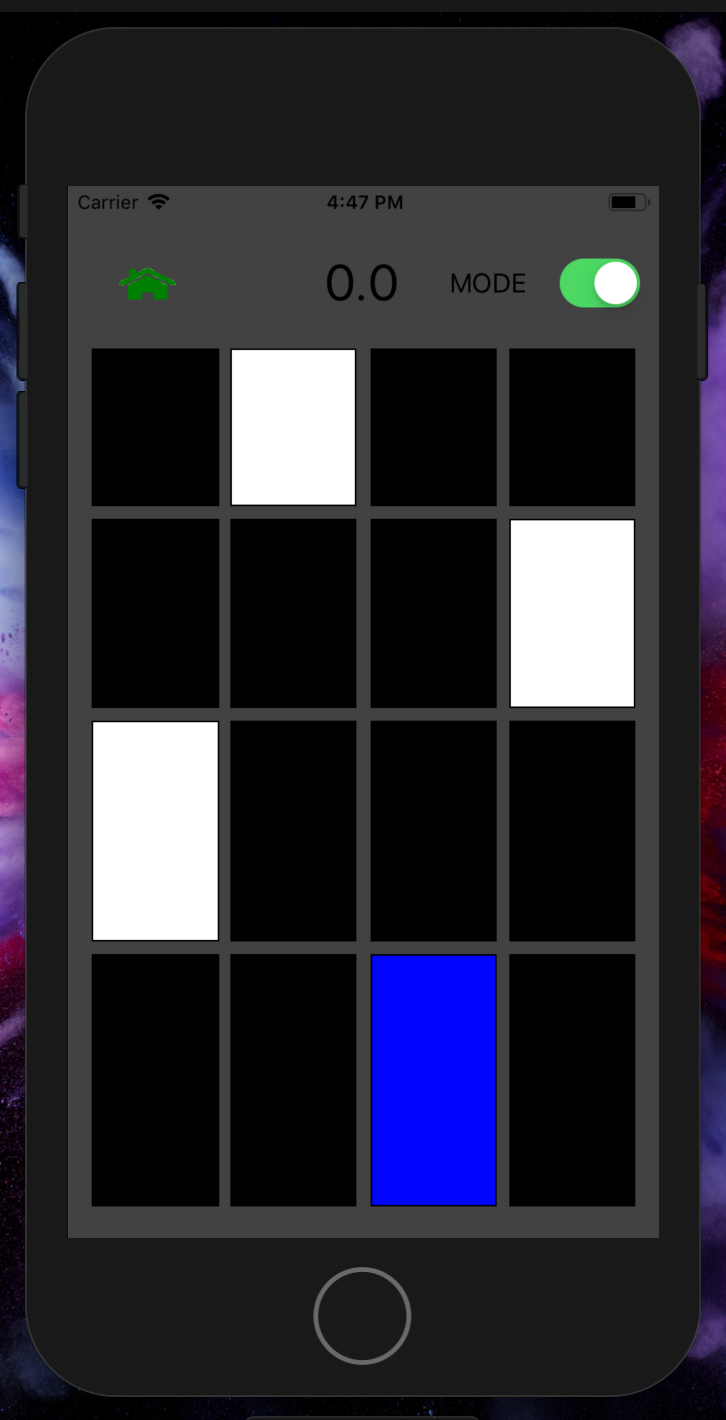
\includegraphics[width=20mm]{iOSapp1}
      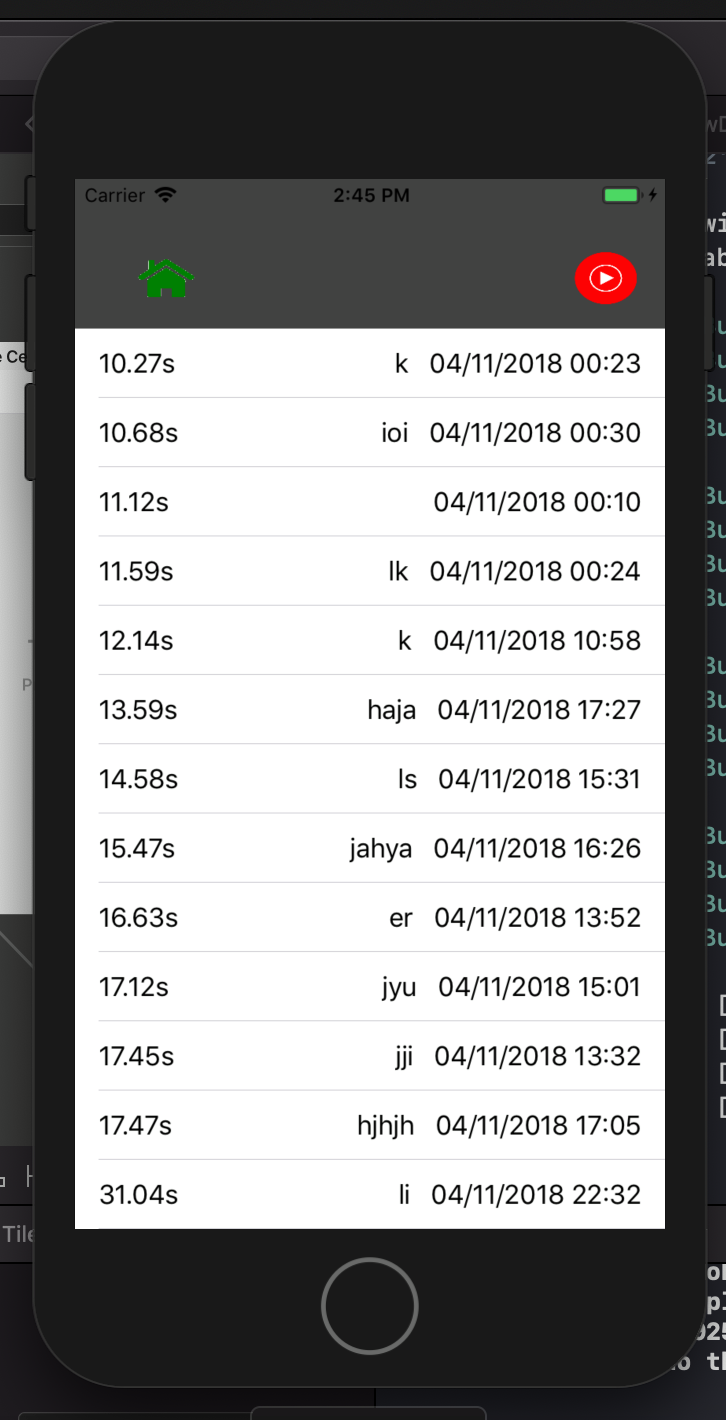
\includegraphics[width=20mm]{iOS}

    \end{center}
    \end{itemize}
  \end{block}

\end{frame}

%---------------------------------------------------------------------------------------------------------------------------------------------------------
\section{Android}
%---------------------------------------------------------------------------------------------------------------------------------------------------------

\begin{frame}
    \frametitle<1->{Android}
     \begin{block}<1->{Les Activités}
	Il y a 7 \textit{activités}:
{\scriptsize
	\begin{itemize}
	     \item <1->\textit{Accueil} : L'écran d'accueil, apparaît au lancement de l'application. 

	     \item <2->\textit{Game} : Elle permet de lancer le jeu.

	     \item <3->\textit{ResultatNeg} : Elle s'affiche en cas de défaite, on affche le meilleur score s'il y en un. 
On donne ensuite la possibilité au joueur de rejouer ou d'accéder à l'écran d'accueil.

 	     \item <4->\textit{ResultatPos} :  Elle s'affiche en cas de victoire, on affche le meilleur score s'il y en un.
On donne ensuite la possibilité au joueur de rejouer, d'enregistrer son score ou d'accéder à l'écran d'accueil.
on récupère les données transmises par l'activité Game dans l'intent et on les retransmet ensuite pour l'activité
Enregistrer si on appuie sur ce bouton.

	     \item <5->\textit{Enregistrer} : Dans cette activité, on dispose de trois boutons, l'un pour valider son enregistrement, un autre
pour prendre une photo et un autre pour annuler ( pour revenir au menu).
Le joueur a la possibilité d'écrire son nom, mais ne doit pas dépasser une quinzaine de caractères, et doit en entrer au moins trois. 
Les données seront également transmises à l'activité ListeScores.

	     \item <6->\textit{ListeScore} : Dans cette activité, nous allons créer les scores, les afficher et les enregistrer dans une base de données (via les classes Score, ScoresAdapter et MyDBAdapter)

	     \item <7->\textit{Maps} : Cette activité permet à  l’application de récupérer la position du joueur et l’afficher sur une
carte.

	\end{itemize} 
}

     \end{block}

\end{frame}

%------------------------------------------------
\begin{frame}
\frametitle{Android}
\begin{block}{Activity Game}
	L'objectif ici était de pouvoir ajouter une couleur aux boutons pour simuler des touches de
piano. Ainsi, dès que cette activité est lancée, nous générons{ \color{red} un nombre aléatoire compris entre 1
et 4} pour chacune des lignes afin de déterminer quel bouton sera {\color{red} noir}. Les autres seront dès lors
coloriés en blanc .

\end{block}
\end{frame}

%------------------------------------------------

\begin{frame}
\frametitle{Android}
\begin{block}{Activity Game}
	L'objectif ici était de pouvoir ajouter une couleur aux boutons pour simuler des touches de
piano. Ainsi, dès que cette activité est lancée, nous générons{ \color{red} un nombre aléatoire compris entre 1
et 4} pour chacune des lignes afin de déterminer quel bouton sera {\color{red} noir}. Les autres seront dès lors
coloriés en blanc .

\end{block}

    \begin{center}
      
\includegraphics[width=20mm]{AndroidGame}
      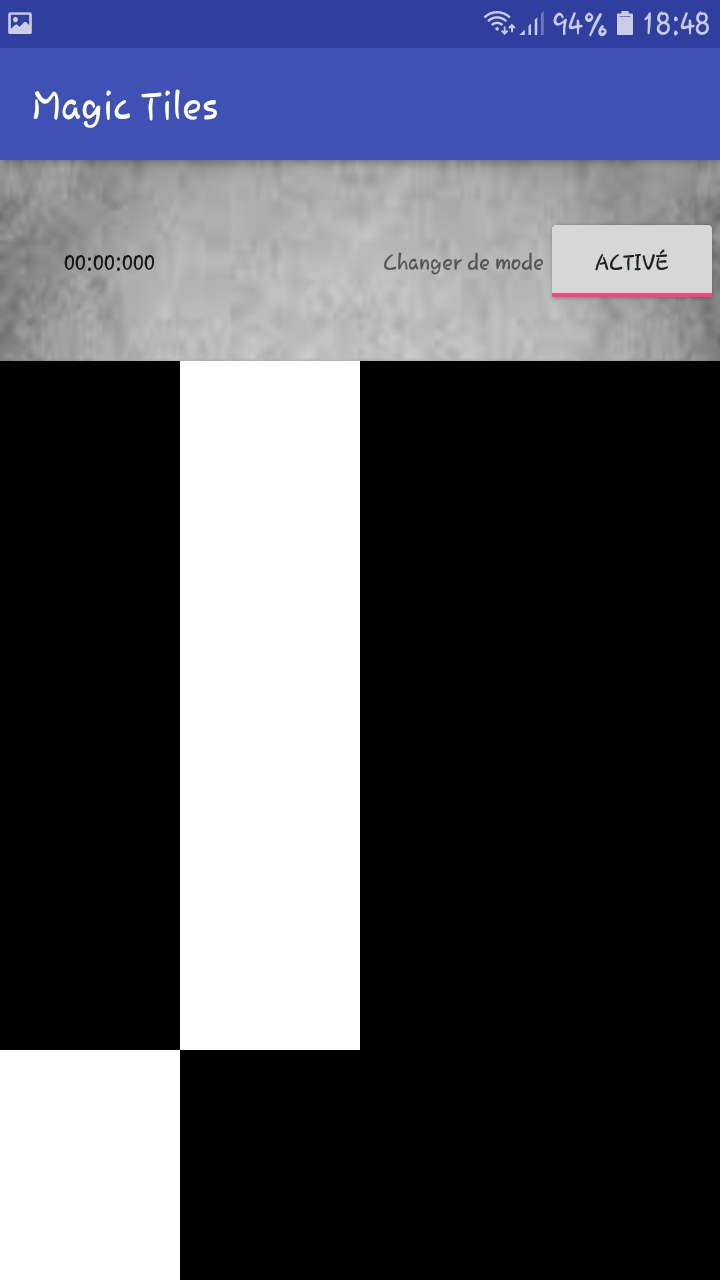
\includegraphics[width=20mm]{AndroidGameInvers}

    \end{center}
   
\end{frame}

%------------------------------------------------

\begin{frame}
\frametitle<1->{Android}
\begin{block}<1->{Activity Game}
	Une seule ligne de boutons est cliquable - nous l'appelleront " {\color{red} Ligne 0} " -, celle qui se situe tout
en bas de l'écran, le reste des boutons sont désactivé. Nous n'avons donc ajouté des écouteurs
qu'aux boutons de la ligne 0.

\end{block}

   \begin{center}Ligne 0 ->
      
\includegraphics[width=20mm]{AndroidGame}
      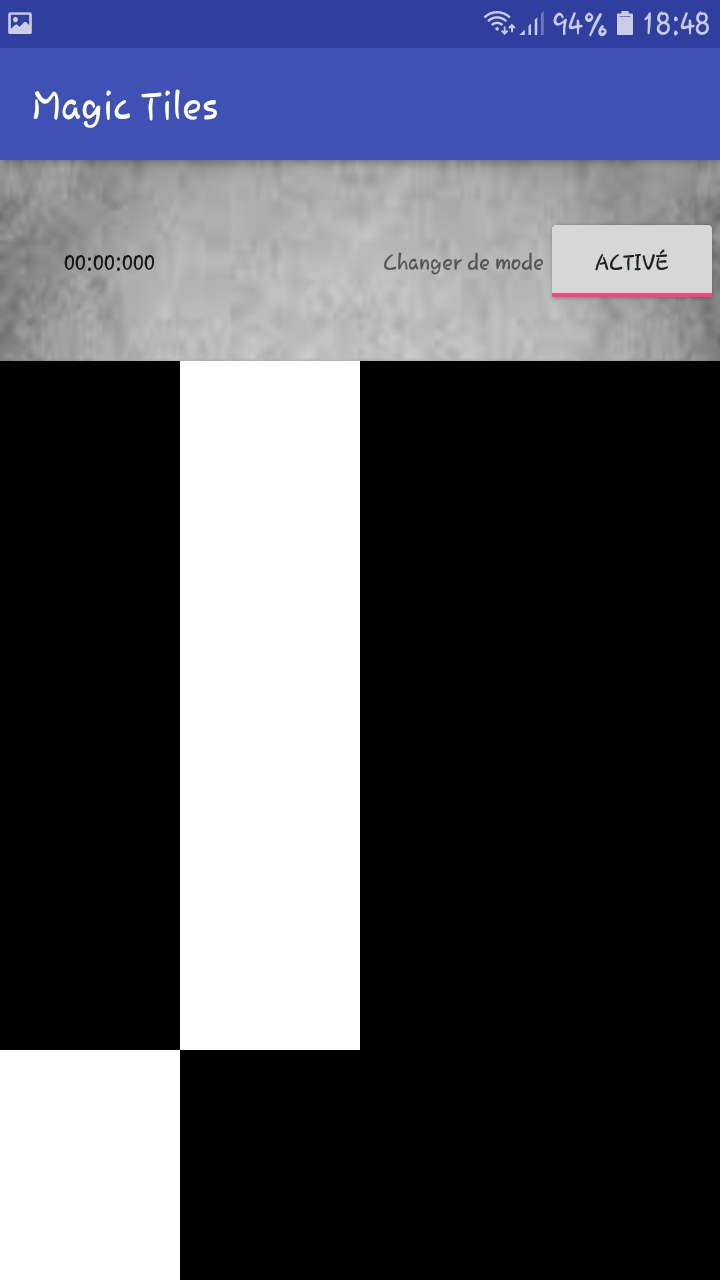
\includegraphics[width=20mm]{AndroidGameInvers}

    \end{center}

\begin{exampleblock}<2->{Activity Game}
	     {\small Lorsqu'on appuie pour la premier fois sur l'un des boutons de la ligne 0,
 { \color {red}le chronomètre sera démarré} et le choix du mode ne sera dès lors {\color {red} plus accessible}.}



\end{exampleblock}
   
\end{frame}

%------------------------------------------------

\begin{frame}
\frametitle<1->{Android}


    \begin{center}
      
\includegraphics[width=20mm]{AndroidGame}
      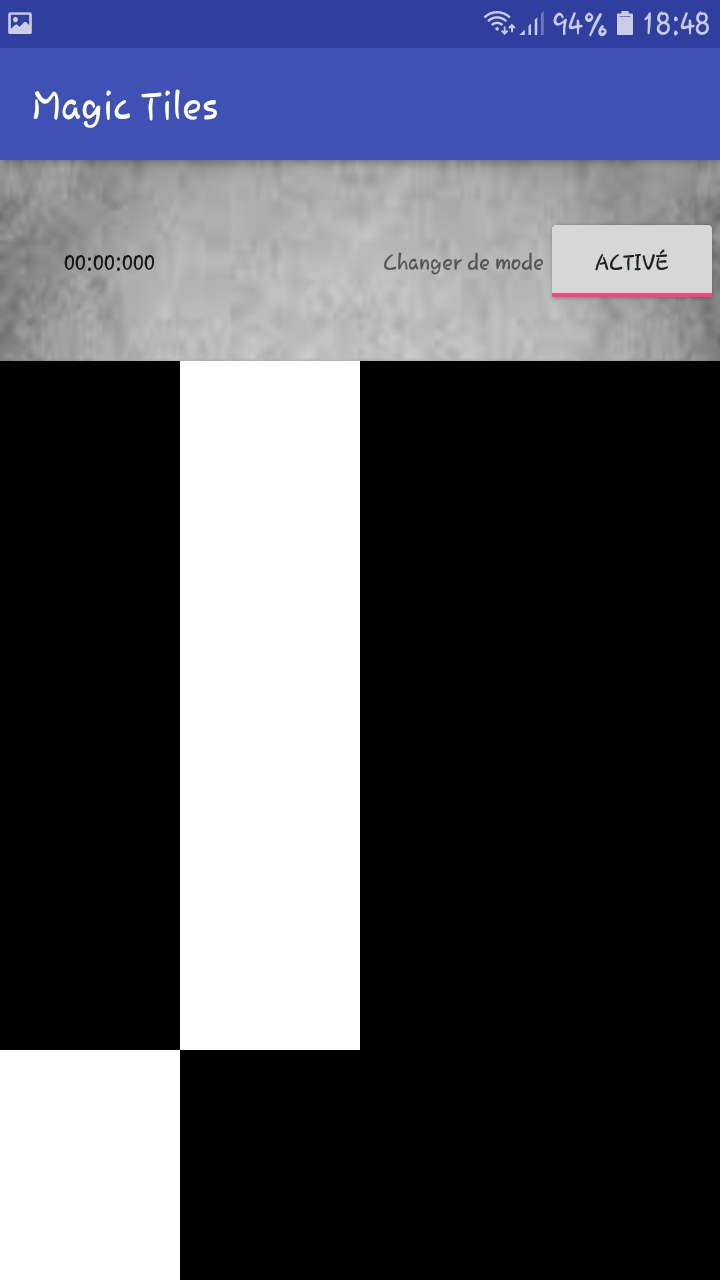
\includegraphics[width=20mm]{AndroidGameInvers}

    \end{center}
   
\end{frame}




%---------------------------------------------------------------------------------------------------------------------------------------------------------
\section{iOS}
%---------------------------------------------------------------------------------------------------------------------------------------------------------



%---------------------------------------------------------------------------------------------------------------------------------------------------------
\section{Démonstration}
%---------------------------------------------------------------------------------------------------------------------------------------------------------

\begin{frame}
\frametitle{Démonstration}
	\Huge{\centerline{Démonstration}}
\end{frame}

%---------------------------------------------------------------------------------------------------------------------------------------------------------
\section{Conclusion}
%---------------------------------------------------------------------------------------------------------------------------------------------------------


\begin{frame}
\frametitle{Conclusion}
	\begin{block}{Conclusion}
	Ce projet a fait l'objet d'une expérience à  la fois intéressante et enrichissante, qui nous a permis d'améliorer nos connaissances et nos compétences dans le domaine du développement d'applications mobile.
	\end{block}
\end{frame}

\begin{frame}
\Huge{\centerline{The End}}
\end{frame}

%----------------------------------------------------------------------------------------

\end{document} 